%% TALS Schieberegler im CAS-Rechner

\paragraph{Schieberegler}\index{Schieberegler} Der Taschenrechner \textit{TI-$n$Spire CX
  II-T CAS} kann Terme in der Variablen $x$ parametrisiert
darstellen. Erstellen Sie dazu in einem Dokument eine
\textit{notes}-Page und definieren Sie den Term $terma := a\cdot
x+0.5$. In einem neuen Grafik-Fenster (Page) zum selben Problem
definieren Sie die Funktion $f1(x):=terma$. Damit erscheint die Frage
nach einem Schieberegler, welcher uns den Parameter $a$ verändern
lassen kann.

\bbwCenterGraphic{6cm}{allg/gleichungen/img/LineareFunktionTR_terma.png}
%  \begin{center}
%   \raisebox{-1cm}{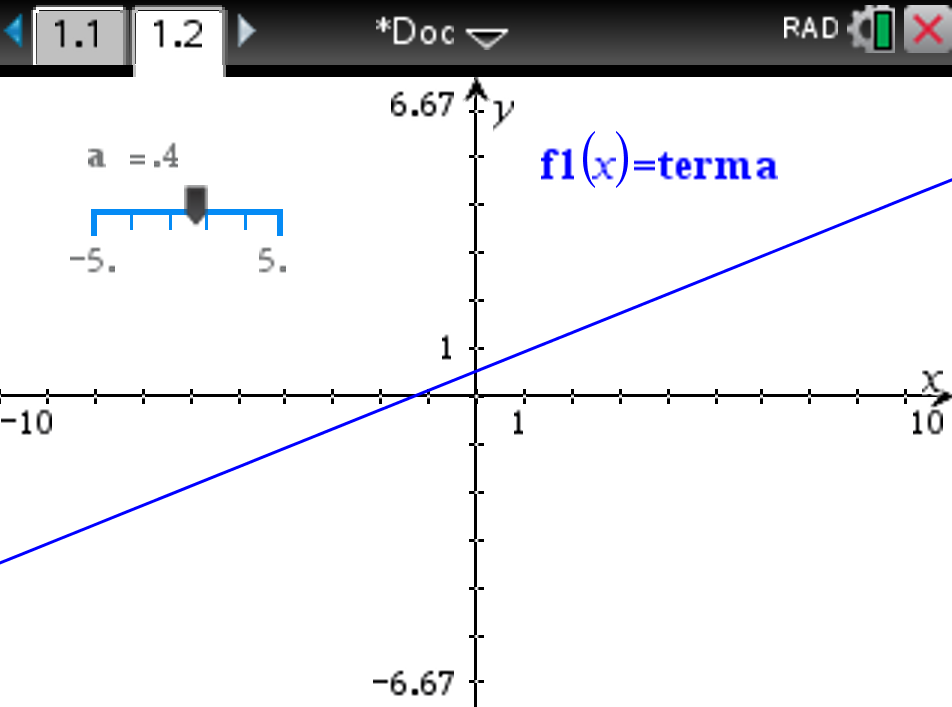
\includegraphics[width=6cm]{img/LineareFunktionTR_terma.png}}
%  \end{center}


\paragraph{Frage 1} Bei welchem Parameter $b$ hat die folgende Gleichung für $x$ die Lösung $1.5$?
$$-2x + b = 0$$

\noTRAINER{$$.....................................$$}
\TRAINER{$$b = 3$$}
Dies lösen wir, indem wir die gesuchte Lösung für $x$ einsetzen und nach $b$ auf"|lösen. Graphisch kann dies auch mit dem CAS-Rechner \textit{gelöst} werden. Definieren Sie «termb := $-2\cdot{}x+b$» und zeichnen Sie den Graphen in einer Graph-Page.
Erstellen Sie einen «Slider»\index{Slider}\index{Schieberegler} für $b$ und ziehen Sie an
diesem \textit{Slider}, bis der Wert der Geraden auf der $x$-Achse den
Wert 1.5 (gesuchte Lösung) angenähert hat.


\paragraph{Frage 2} Bei welchem Parameter $b$ hat die folgende Gleichung für $x$ die Lösung $1.5$?
$$ax-3=0$$

\noTRAINER{$$.....................................$$}
\TRAINER{$$a=2$$}
Dies nähern wir auch mit dem CAS-Rechner an. Definieren Sie den Term
$terma$ neu ($terma := a\cdot{}x-3$) und zeichnen Sie den Graphen in einer Graph-Page.
Ziehen Sie am \textit{Slider}, bis der Wert der Geraden auf der
$x$-Achse dem Wert 1.5 (gesuchte Lösung) genug nahe kommt.
